\documentclass{beamer}
% \usetheme{default}
\usetheme{Boadilla}
\usepackage[utf8x]{inputenc}
\usepackage{default}
\usepackage{amsmath,amsthm,amsfonts,amssymb,graphicx,xcolor,ifthen}
\usepackage{algorithm,listings}
\usepackage{algorithmicx,algpseudocode}
\usepackage{multirow,array,lscape,chngpage,rotating}
\usepackage{colortbl,calc,fp}

\usepackage{tikz}
\usepackage{pgfplots}
\usetikzlibrary{snakes,patterns,shapes,calc}

%%%%%%%%%%%%%%%%%%%%%%%%%%%%%%%%%%%%%%%%

\DeclareMathOperator*{\argmin}{arg\,min}
\DeclareMathOperator*{\argmax}{arg\,max}
\DeclareMathOperator*{\vectorize}{vec}

\newcommand{\normal}[2]{\ensuremath{\mathcal{N}\left({{#1}},{{#2}}\right)}}
\newcommand{\trans}[1]{\ensuremath{{#1}^{\mathsf{T}}}}

\newcommand{\e}{\mathbf{e}}
\newcommand{\bb}{\mathbf{k}}
\newcommand{\kL}{\mathbf{k}^L}
\newcommand{\kG}{\mathbf{k}^G}
%\newcommand{\uu^m}{\mathbf{w}}
\newcommand{\x}{\mathbf{x}}
\newcommand{\y}{\mathbf{y}}
\newcommand{\uu}{\mathbf{u}}
\newcommand{\vv}{\mathbf{v}}
\newcommand{\timestep}{s}

\newcommand{\fixme}[1]{\textbf{FIXME: {#1}}}
\newcommand{\new}[1]{\color{red} {#1}}

\definecolor{darkgreen}{RGB}{0,127,0}

%%%%%%%%%%%%%%%%%%%%%%%%%%%%%%%%%%%%%%%
\author {Mike Izbicki}
\institute{UC Riverside}
\title[Identifying Attacks in Power Systems]{}

\newcommand \imgpath[1]{/home/user/docs/phd/presentation_lib/{#1}}


\AtBeginSection[]
{
  \begin{frame}<beamer>
    \frametitle{Outline for section \thesection}
    \tableofcontents[currentsection]
  \end{frame}
}

%%%%%%%%%%%%%%%%%%%%%%%%%%%%%%%%%%%%%%%%%%%%%%%%%%%%%%%%%%%%%%%%%%%%%%%%%%%%%%%%

\begin{document}
\beamertemplatenavigationsymbolsempty

%%%%%%%%%%%%%%%%%%%%%%%%%%%%%%%%%%%%%%%%

\begin{frame}
\begin{center}
\Huge
Identification of Destabilizing Attacks 
in Power Systems
\end{center}

\vspace{0.5in}
\begin{center}
\textbf{Mike Izbicki}, Sajjad Amini, Christian R. Shelton, Hamed Mohsenian-Rad

UC Riverside
\end{center}
\end{frame}

%%%%%%%%%%%%%%%%%%%%%%%%%%%%%%%%%%%%%%%%

\begin{frame}[fragile]{What is a destabilizing attack? (and why you should care?)}

%\vspace{-0.045in}

\begin{center}
\begin{tikzpicture}[scale=0.9]
\small

%\draw[blue,line width=0.25pt,fill,draw opacity=0.5,fill opacity=0.1]
    %(-3.95,0.8) -- (-2.75,0.8) -- (-2.75,1.9) -- (-3.95,1.9) -- cycle;
    %(-4.85,0.8) -- (-3.65,0.8) -- (-3.65,1.9) -- (-4.85,1.9) -- cycle;

%\draw[dotted,thick] (-3.95,1.9) -- (-4.1,3.6);
%\draw[dotted,thick] (-2.75,1.9) -- (4.1,3.6);

\node[rectangle,align=center] at (4,-0.75) {standard IEEE \\ 9 bus power system};
\uncover<2>{
\node at (4,-1.5) { (\textcolor{darkgreen}{normal operations}) };
}
\uncover<3>{
\node at (4,-1.5) { (\textcolor{red}{static attack}) };
}
\uncover<4-7>{
\node at (4,-1.5) { (\textcolor{red}{dynamic attack}) };
}

%\node[rectangle,align=center] at (5.2 ,4.8) {\rotatebox{90}{Rotor Angle}};
%\node[rectangle,align=center] at (4.85,4.8) {\rotatebox{90}{Frequency}};
%\node[rectangle,align=center] at (4.5 ,4.8) {\rotatebox{90}{Deviation}};

\uncover<2-7>{
\node[rectangle,align=center] at (5.5 ,6.0) {\color{blue} rotor angle};
\node[rectangle,align=center] at (5.5 ,5.55) {\color{blue} frequency};
\node[rectangle,align=center] at (5.5 ,5.10) {\color{blue} deviation};

\node[rectangle,align=center] at (5.95 ,3.50) {\color{purple} bus load (kW)};

%\node at (0,10) {};
\node at (0,5.5) {
    \begin{tikzpicture}[scale=0.9]

    \draw[fill=green,draw opacity=0,fill opacity=0.05] (0,0.3) -- (8.20,0.3) -- (8.20,1.95) -- (0,1.95);
    \draw[dashed,darkgreen] (0,0.3) -- (8.2,0.3);
    \draw[dashed,darkgreen] (8.2,1.95) -- (0,1.95);

    \node at (3.25,0.5) {\color{darkgreen} safe operating range};
    \uncover<2>{
    \begin{axis}
        [ domain=-30:80
        , xmin=-30
        , xmax=80
        , ymin=-2000
        , ymax=2000
        , width=3.85in
        , height=1.5in
        , samples=500
        , xtickmin=1,xtickmax=0,ytickmin=1,ytickmax=0, minor tick num=0, scaled ticks=false, xticklabel=\empty,yticklabel=\empty
        ]
    \draw[ultra thin,opacity=0.2] (axis cs:\pgfkeysvalueof{/pgfplots/xmin},0) -- (axis cs:\pgfkeysvalueof{/pgfplots/xmax},0);
    \addplot[color=blue,mark=none] {0};
    \end{axis}
    }
    \uncover<3>{
    \begin{axis}
        [ domain=-30:80
        , xmin=-30
        , xmax=80
        , ymin=-2000
        , ymax=2000
        , width=3.85in
        , height=1.5in
        , samples=500
        , xtickmin=1,xtickmax=0,ytickmin=1,ytickmax=0, minor tick num=0, scaled ticks=false, xticklabel=\empty,yticklabel=\empty
        ]
    \draw[ultra thin,opacity=0.2] (axis cs:\pgfkeysvalueof{/pgfplots/xmin},0) -- (axis cs:\pgfkeysvalueof{/pgfplots/xmax},0);
    \addplot[color=blue,mark=none] {(\x>0)*2000*(x/4)^(0.5)*exp(-(x/4)^(1.5))};
    \end{axis}
    }
    \uncover<4-7>{
    \begin{axis}
        [ domain=-30:80
        , xmin=-30
        , xmax=80
        , ymin=-2000
        , ymax=2000
        , width=3.85in
        , height=1.5in
        , samples=500
        , xtickmin=1,xtickmax=0,ytickmin=1,ytickmax=0, minor tick num=0, scaled ticks=false, xticklabel=\empty,yticklabel=\empty
        ]
    \draw[ultra thin,opacity=0.2] (axis cs:\pgfkeysvalueof{/pgfplots/xmin},0) -- (axis cs:\pgfkeysvalueof{/pgfplots/xmax},0);
    \addplot[color=blue,mark=none] {(\x>0)*x^(1.75)*sin(deg(x))};
    \end{axis}
    }

    \end{tikzpicture}
};
\node at (0,3.5) {
    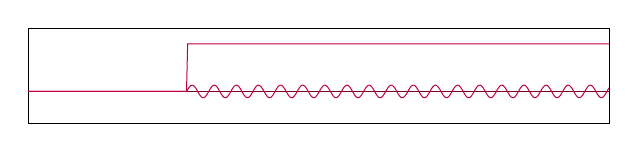
\begin{tikzpicture}[scale=0.9]
    \uncover<2>{
    \begin{axis}
        [ domain=-30:80
        , xmin=-30
        , xmax=80
        , ymin=-1000
        , ymax=2000
        , width=3.85in
        , height=1.15in
        , samples=500
        , xtickmin=1,xtickmax=0,ytickmin=1,ytickmax=0, minor tick num=0, scaled ticks=false, xticklabel=\empty,yticklabel=\empty
        ]
    \draw[ultra thin,opacity=0.2] (axis cs:\pgfkeysvalueof{/pgfplots/xmin},0) -- (axis cs:\pgfkeysvalueof{/pgfplots/xmax},0);
    \addplot[color=purple,mark=none] {0};
    \end{axis}
    }
    \uncover<3>{
    \begin{axis}
        [ domain=-30:80
        , xmin=-30
        , xmax=80
        , ymin=-1000
        , ymax=2000
        , width=3.85in
        , height=1.15in
        , samples=500
        , xtickmin=1,xtickmax=0,ytickmin=1,ytickmax=0, minor tick num=0, scaled ticks=false, xticklabel=\empty,yticklabel=\empty
        ]
    \draw[ultra thin,opacity=0.2] (axis cs:\pgfkeysvalueof{/pgfplots/xmin},0) -- (axis cs:\pgfkeysvalueof{/pgfplots/xmax},0);
    \addplot[color=purple,mark=none] {(\x>0)*1500};
    \end{axis}
    }
    \uncover<4-7>{
    \begin{axis}
        [ domain=-30:80
        , xmin=-30
        , xmax=80
        , ymin=-1000
        , ymax=2000
        , width=3.85in
        , height=1.15in
        , samples=500
        , xtickmin=1,xtickmax=0,ytickmin=1,ytickmax=0, minor tick num=0, scaled ticks=false, xticklabel=\empty,yticklabel=\empty
        ]
    \draw[ultra thin,opacity=0.2] (axis cs:\pgfkeysvalueof{/pgfplots/xmin},0) -- (axis cs:\pgfkeysvalueof{/pgfplots/xmax},0);
    \addplot[color=purple,mark=none] {(\x>0)*200*sin(deg(1.5*x))};
    \end{axis}
    }
    \end{tikzpicture}
};
}

\node at (0,0) {
    \includegraphics[width=2.7in]{img/IEEE9}
    %\includegraphics[width=3in]{img/IEEE9}
    %\includegraphics[width=0.8\textwidth,height=1.7in]{img/IEEE9}
};

\uncover<2-7>{
\node[draw=purple,fill=purple,fill opacity=0.05,circle,minimum width=1.5cm] (8) at (0.25,1.6) {};
\draw[->,draw=purple,thick] (-0.55,1.8) to[in=270,out=150] (-1.5,2.75);

\node[draw=blue,fill=blue,fill opacity=0.05,circle,minimum width=1.5cm] at (-3.25,1.25) {};
\draw[->,draw=blue,thick] (-4.05,1.6) to[in=225,out=150] (-4.25,5.25);
}

\uncover<5-7>{
\node[draw=red,fill=red,fill opacity=0.05,circle,minimum width=1.5cm] (3) at (3.5,1.25) {};
\draw[red,thick,->] (3) to[out=120,in=20] (8);

\node[rectangle,align=center] at (5.25,1) {\color{red}positive \\\color{red}feedback};
%\node at (4,-0.35) {\color{red}between unrelated nodes};
}

\uncover<6-7>{
\node[minimum width=4.55in,minimum height=0.5in,draw=blue,rectangle,rounded corners=0.5cm,fill=white] at (0.25in,-0.8) {};
\node[minimum width=4.55in,minimum height=0.5in,draw=blue,rectangle,rounded corners=0.5cm,fill=blue,opacity=0.05] at (0.25in,-0.8) {};
}
\uncover<6>{
\node[minimum width=4.55in,minimum height=0.5in,draw=blue,rectangle,rounded corners=0.5cm,align=left] at (0.25in,-0.8) 
    { \normalsize \textbf{Previous work:} detects the presence of an attack 
    };
}
\uncover<7>{
\node[minimum width=4.55in,minimum height=0.5in,draw=blue,rectangle,rounded corners=0.5cm,align=left] at (0.25in,-0.8) 
    { \normalsize \textbf{Our work:} identify which bus is attacked (so we can isolate it)
    };
}


\end{tikzpicture}
\end{center}

\end{frame}



%%%%%%%%%%%%%%%%%%%%%%%%%%%%%%%%%%%%%%%%

\begin{frame}{Outline}
\Large
\begin{itemize}
\item Power system dynamics
\begin{itemize}
\Large
\item Normal operation
\item Under attack
\end{itemize}

\vspace{0.15in}
\item Identifying the attack 
\begin{itemize}
\Large
\item Unscented Kalman Filter (UKF)
\item Joint state and variable estimation

\vspace{0.075in}
\item Rank-1 approximate filter (our contribution)
\begin{itemize}
\Large
\item Reduces computational complexity
\item Improves statistical efficiency
\end{itemize}
\end{itemize}

\vspace{0.15in}
\item Simulation results
\end{itemize}
\end{frame}

%%%%%%%%%%%%%%%%%%%%%%%%%%%%%%%%%%%%%%%%

\begin{frame}{System dynamics under normal conditions}
With $g$ generators and $\ell$ loads, model the power grid as:
\begin{equation}
\label{eq:discrete}
\x_{t+1} = A\x_t + B\uu_t + \epsilon.
%\x_{t+1} = (\timestep A+I)\x_t + \timestep B\uu_t + \epsilon.
%\x_{t+1} = (\timestep A+sBA^p_t+I)\x_t + \timestep B(\uu_t^n+\uu_t^p) + \epsilon.
\end{equation}
where
\begin{align*}
\x &= 
\text{vector of}
\begin{cases}
\text{$g$ generator voltage phase angles} \\
\text{$g$ generator rotor angular frequency deviation} \\
\text{$\ell$ load voltage phase angles} \\
\end{cases} \\
\uu &= \text{vector of} 
\begin{cases}
\text{$g$ power generation at all generator buses} \\
\text{$\ell$ power consumption at all load buses} \\
\end{cases}\\
%\timestep &= \text{step size in seconds} \\
A,B &= \text{highly structured matrices that depend on the grid's connectivity} \\
\epsilon &\sim \mathcal{N}(0,Q) \text{~captures modeling and measurement errors} \\
\end{align*}
\end{frame}

%%%%%%%%%%%%%%%%%%%%%%%%%%%%%%%%%%%%%%%%%%%%%%%%%%%%%%%%%%%%%%%%%%%%%%%%%%%%%%%%

\begin{frame}{System dynamics under attack}
Decompose the control into normal $(\uu^n)$ and attack $(\uu^a)$ components:
\begin{equation}
\uu = \uu^n + \uu^a.
\end{equation}
Assume the attacker uses a proportional controller
\begin{equation}
\uu^a = A^p\x + \uu^p,
%\end{equation}
\text{~~~~~where~~~~~}
%\begin{equation}
A^p =
\begin{bmatrix}
0 & 0 & -(D^L)^{-1}K^{LG}
\\
0 & 0 & 0
\end{bmatrix}
.
\end{equation}
$D^L$ matrix of load damping coefficients (determined by power system).
$K^{LG}_{\ell,g}$ is the gain from the load $\ell$ to generator $g$ (determined by attacker).

\noindent\rule[0.5ex]{\linewidth}{1pt}
\pause

Substituting into the system dynamics gives
\begin{equation}
\x_{t+1} = (A+BA^p)\x_t + B(\uu_t^n+\uu_t^p) + \epsilon.
%\x_{t+1} = (\timestep A+sBA^p+I)\x_t + \timestep B(\uu_t^n+\uu_t^p) + \epsilon.
\end{equation}
\textbf{Our goal:} estimate the $A^p$ matrix given a trajectory of $\x$s.

This tells us which load bus has positive feedback from which generator.

\end{frame}

%%%%%%%%%%%%%%%%%%%%%%%%%%%%%%%%%%%%%%%%%%%%%%%%%%%%%%%%%%%%%%%%%%%%%%%%%%%%%%%%

\begin{frame}{Naive solution: joint estimation with the UKF}

Augment our system dynamics
\begin{equation*}
\x_{t+1} = (A+BA^p)\x_t + B(\uu_t^n+\uu_t^p) + \epsilon
%\x_{t+1} = (\timestep A+sBA^p+I)\x_t + \timestep B(\uu_t^n+\uu_t^p) + \epsilon
\end{equation*}
to include the new state variables
\begin{equation*}
\label{eq:aug}
\begin{aligned}
\begin{split}
\begin{bmatrix}
\x_{t+1} \\
\vectorize K^{LG}_{t+1}
\end{bmatrix}
&=
\begin{bmatrix}
A + BA^p_t & 0 \\
%sA + sBA^p_t + I & 0 \\
0 & I
\end{bmatrix}
\begin{bmatrix}
\x_t \\
\vectorize K^{LG}_t
\end{bmatrix}
%\\&~~~~~~~~~~+
+
\begin{bmatrix}
B & 0\\
%sB & 0\\
0 & I
\end{bmatrix}
\begin{bmatrix}
\uu_t^n + \uu_t^p \\
\uu^{LG}_t
\end{bmatrix}
+
\begin{bmatrix}
\epsilon \\
\epsilon^{LG}
\end{bmatrix}
\end{split}
.
\end{aligned}
\end{equation*}

The resulting system is nonlinear.

We solve it with the Unscented Kalman Filter (UKF).

\noindent\rule[0.5ex]{\linewidth}{1pt}
\pause

Note that:
\begin{itemize}
\item $\x$ has $O(\ell+g)$ components (size of original problem)
\item $K^{LG}$ has $O(\ell g)$ components (size of new problem)
\end{itemize}

\pause
Disadvantages of new problem:
\begin{itemize}
\item Computational cost is $O((\ell g)^3)$, much worse than $O((\ell+g)^3)$
\item Not enough data for statistical efficiency
\end{itemize}
\end{frame}

%%%%%%%%%%%%%%%%%%%%%%%%%%%%%%%%%%%%%%%%%%%%%%%%%%%%%%%%%%%%%%%%%%%%%%%%%%%%%%%%

\begin{frame}{Our solution: joint estimation with rank-1 UKF}
Assume that $K^{LG}$ has rank 1:
\begin{equation*}
K^{LG}_t=\kL_t\trans{\kG}_{t}.
\end{equation*}
This is reasonable because there will typically be few attacks.

Then the system dynamics become
\begin{equation*}
\begin{bmatrix}
\x_{t+1} \\
\kL_{t+1} \\
\kG_{t+1} \\
\end{bmatrix}
=
\begin{bmatrix}
A + BA^p_t & 0 & 0\\
%sA + sBA^p_t + I & 0 & 0\\
0 & I & 0\\
0 & 0 & I
\end{bmatrix}
\begin{bmatrix}
\x_t \\
\kL_{t} \\
\kG_{t} \\
\end{bmatrix}
+
\begin{bmatrix}
B & 0 & 0\\
%sB & 0 & 0\\
0 & I & 0\\
0 & 0 & I\\
\end{bmatrix}
\begin{bmatrix}
\uu_t^n + \uu_t^p \\
\uu^L_t \\
\uu^G_t
\end{bmatrix}
+
\begin{bmatrix}
\epsilon \\
\epsilon^K \\
\epsilon^L
\end{bmatrix}
.
\end{equation*}
Solve the system using the UKF.

\noindent\rule[0.5ex]{\linewidth}{1pt}
\pause

Note that:
\begin{itemize}
\item The size of the new state space is $O(\ell+g)$
\item Computationally and statistically efficient
\end{itemize}

\end{frame}

\begin{frame}{Simulation results (statistical efficiency)}
Simulated attack on power system with 100 generators and 100 loads
\vspace{0.075in}

\begin{tikzpicture}
\small
%\node at (8.35,-0.25) {
    %%\rotatebox{90}{$f_i(t)$}
    %\rotatebox{90}{standard method}
    %};
%
%\node at (8.35,3.6) {
    %%\rotatebox{90}{$f_i(t)$}
    %\rotatebox{90}{proposed rank-1 method}
    %};

\node at (-9,0) {
    \rotatebox{90}{entries of $K^{LG}$}
};
%\draw (-9,-2) -- (-9,-0.5);
%\draw[->] (-9,0.5) -- (-9,1.3);

\uncover<1>{
\node at (-0,-0.25) {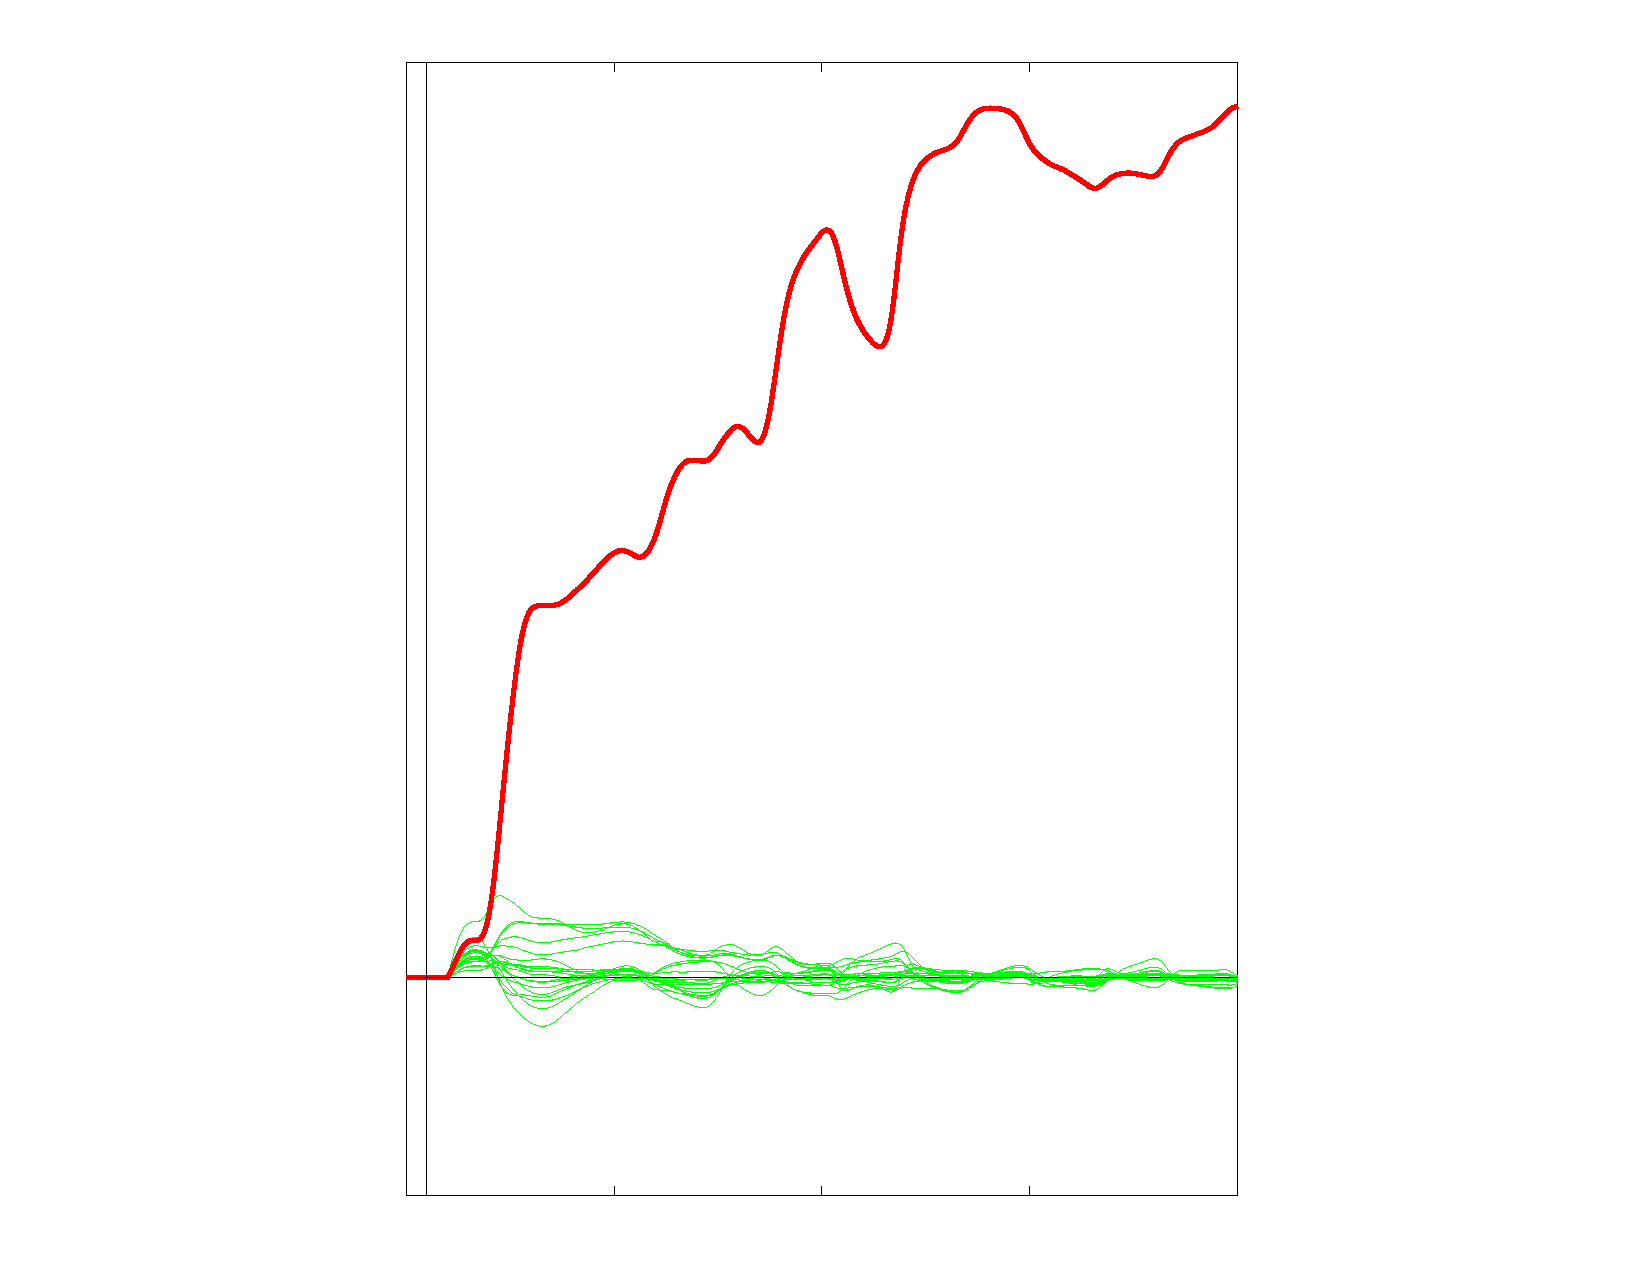
\includegraphics[trim={6.5cm 1cm 5cm 1cm},clip,width=6cm,height=3.5cm]{img/409-clusterSmallWorld-20-addUniform-40-spike-gaussian-Unobserved-rank1-ukf-Xhat}};
\node at (-5.5,-0.25) {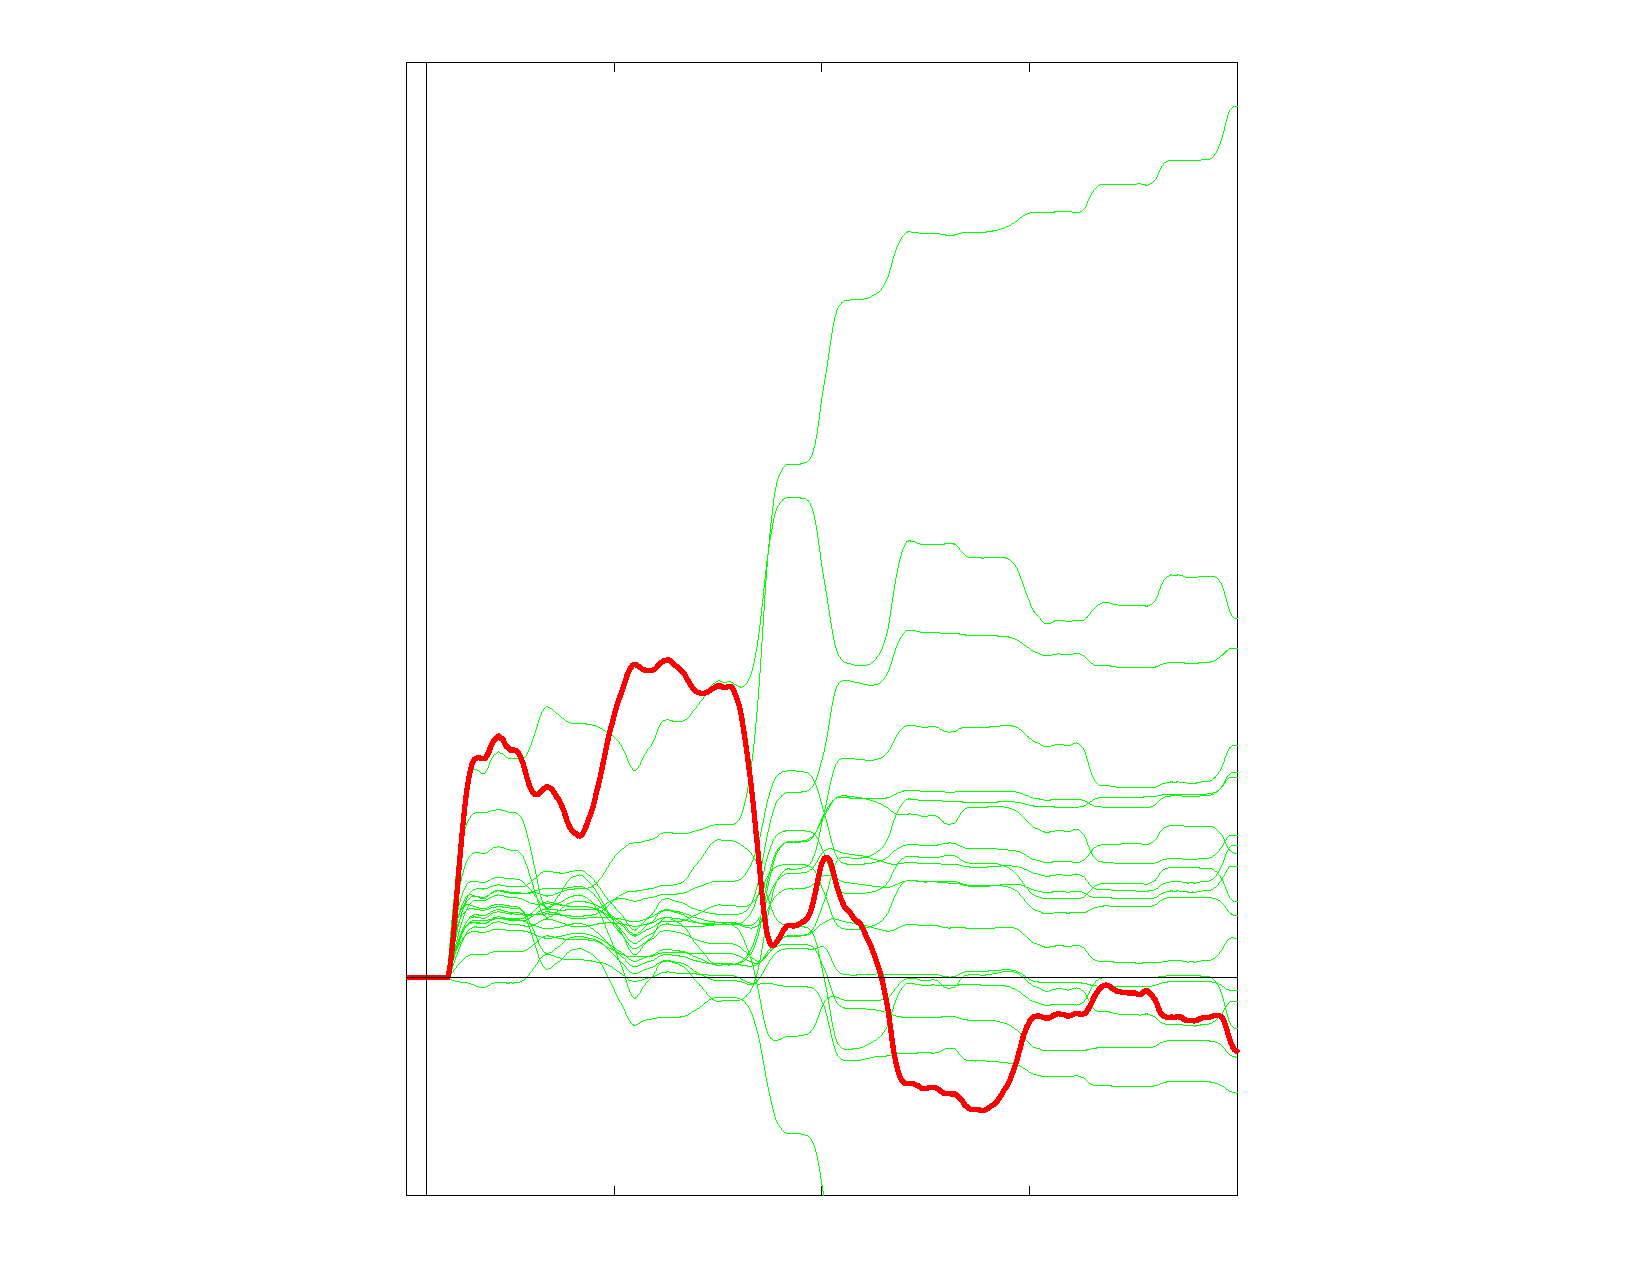
\includegraphics[trim={6.5cm 1cm 5cm 1cm},clip,width=6cm,height=3.5cm]{img/409-clusterSmallWorld-20-addUniform-40-spike-gaussian-Unobserved-fullKL-ukf-Xhat}};
}

\uncover<2>{
\node at (0,-0.25) {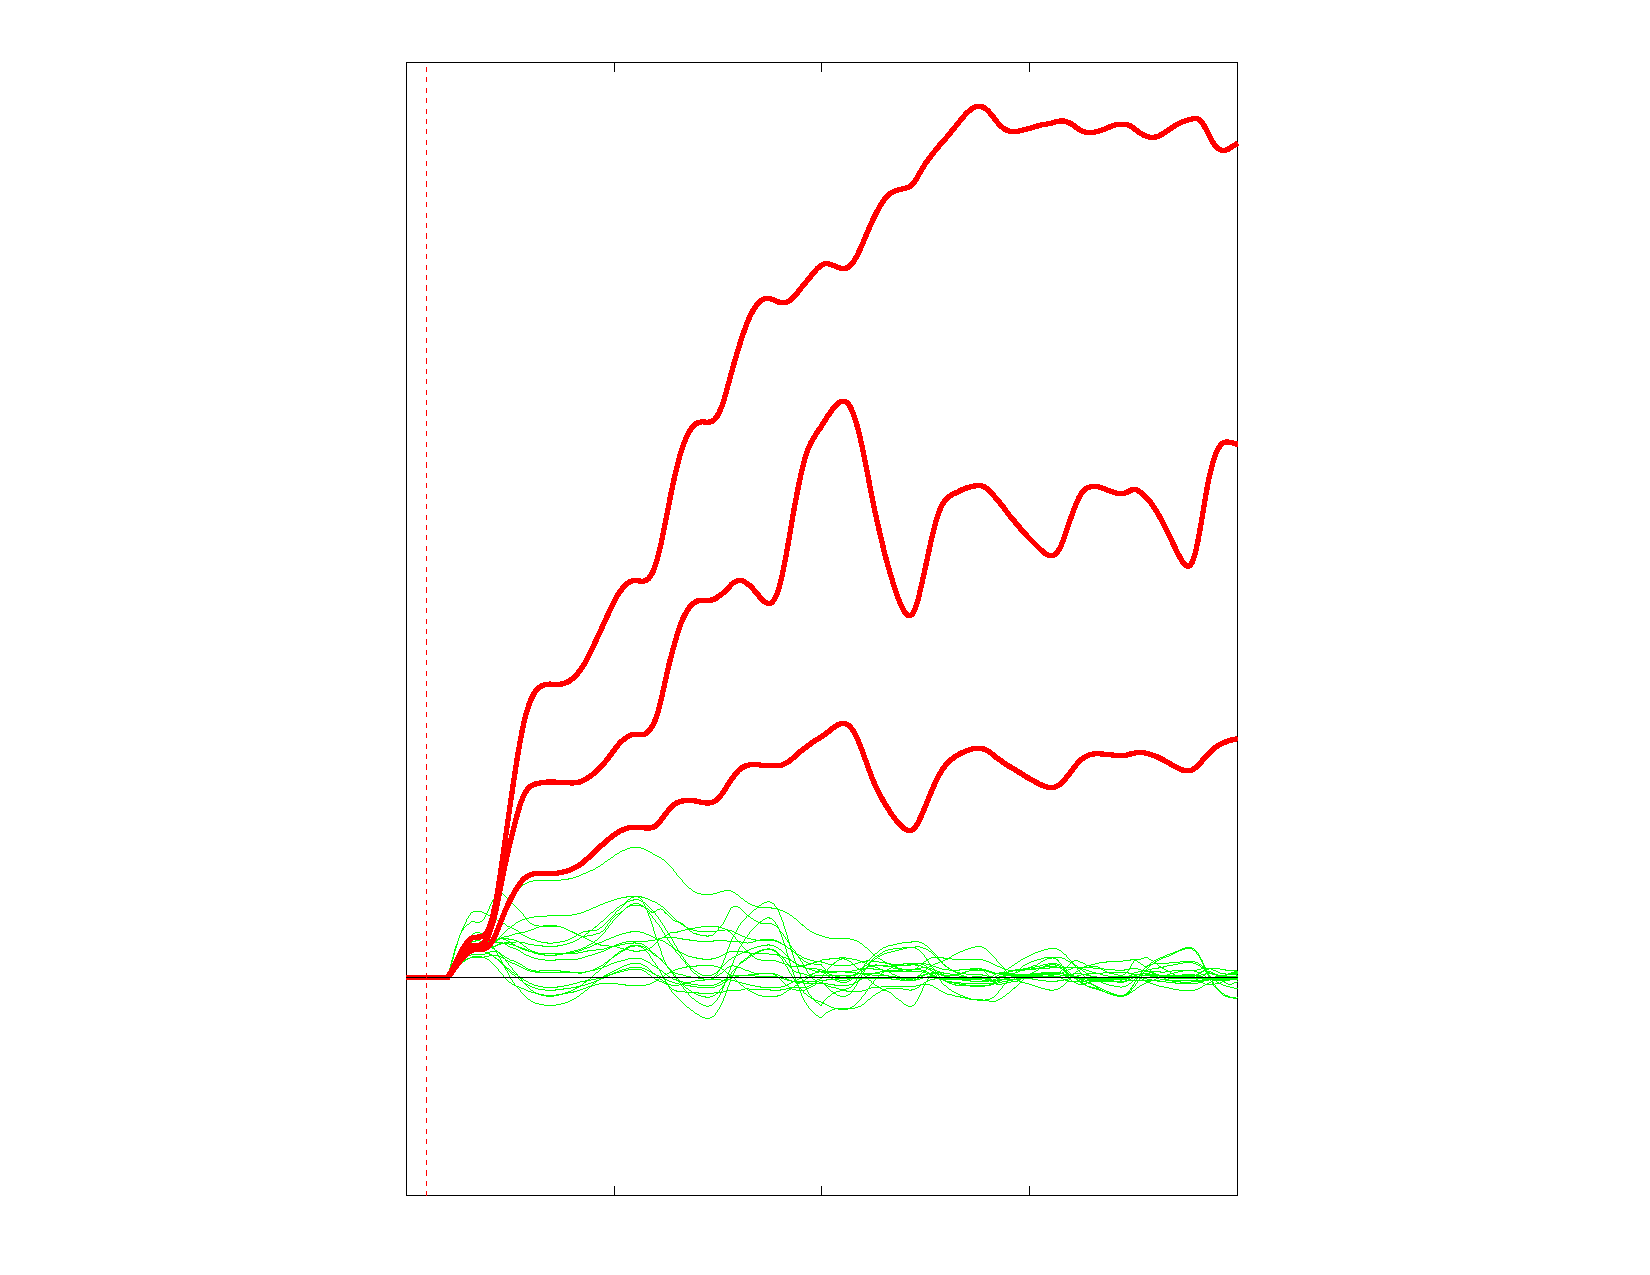
\includegraphics[trim={6.5cm 1cm 5cm 1cm},clip,width=6cm,height=3.5cm]{img/409-clusterSmallWorld-20-addUniform-40-spike3-gaussian-Unobserved-rank1-ukf-Xhat}};
\node at (-5.5,-0.25) {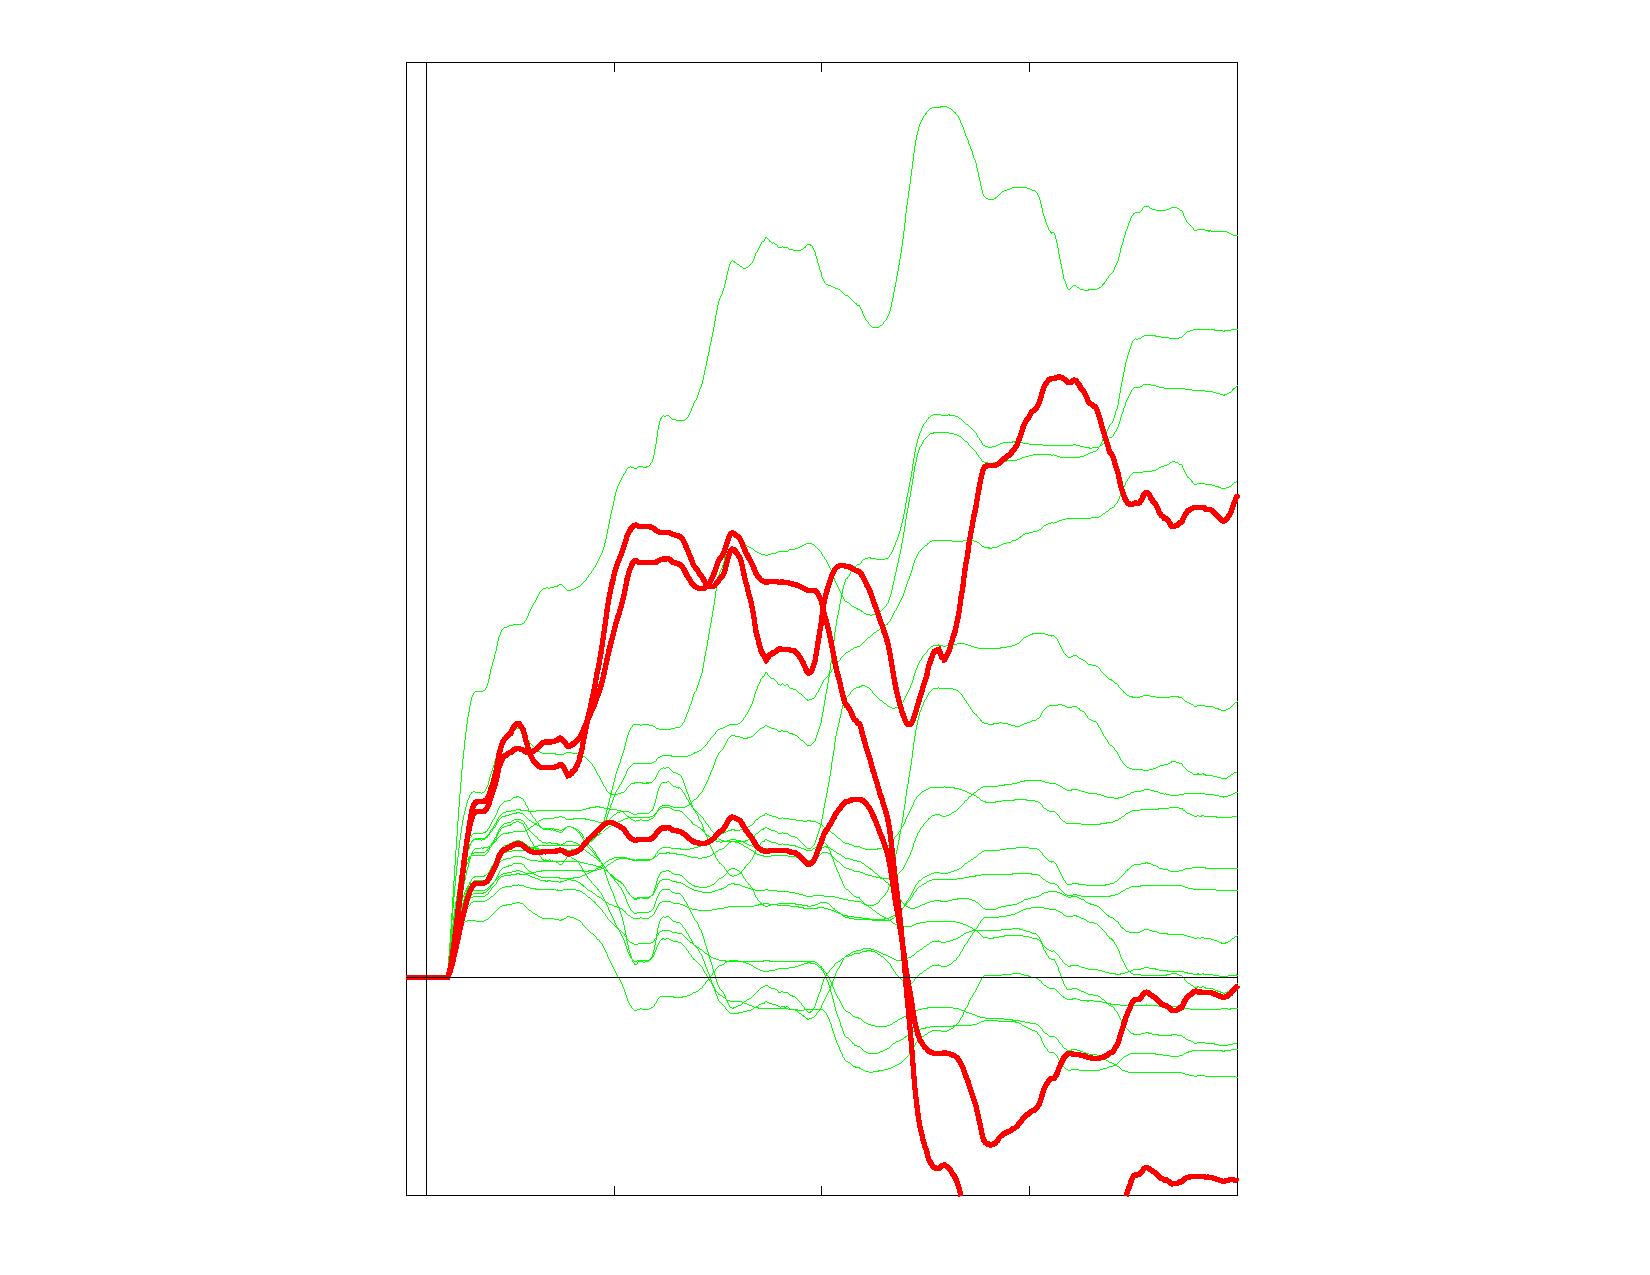
\includegraphics[trim={6.5cm 1cm 5cm 1cm},clip,width=6cm,height=3.5cm]{img/409-clusterSmallWorld-20-addUniform-40-spike3-gaussian-Unobserved-fullKL-ukf-Xhat}};
}

\uncover<3>{
\node at (0,-0.25) {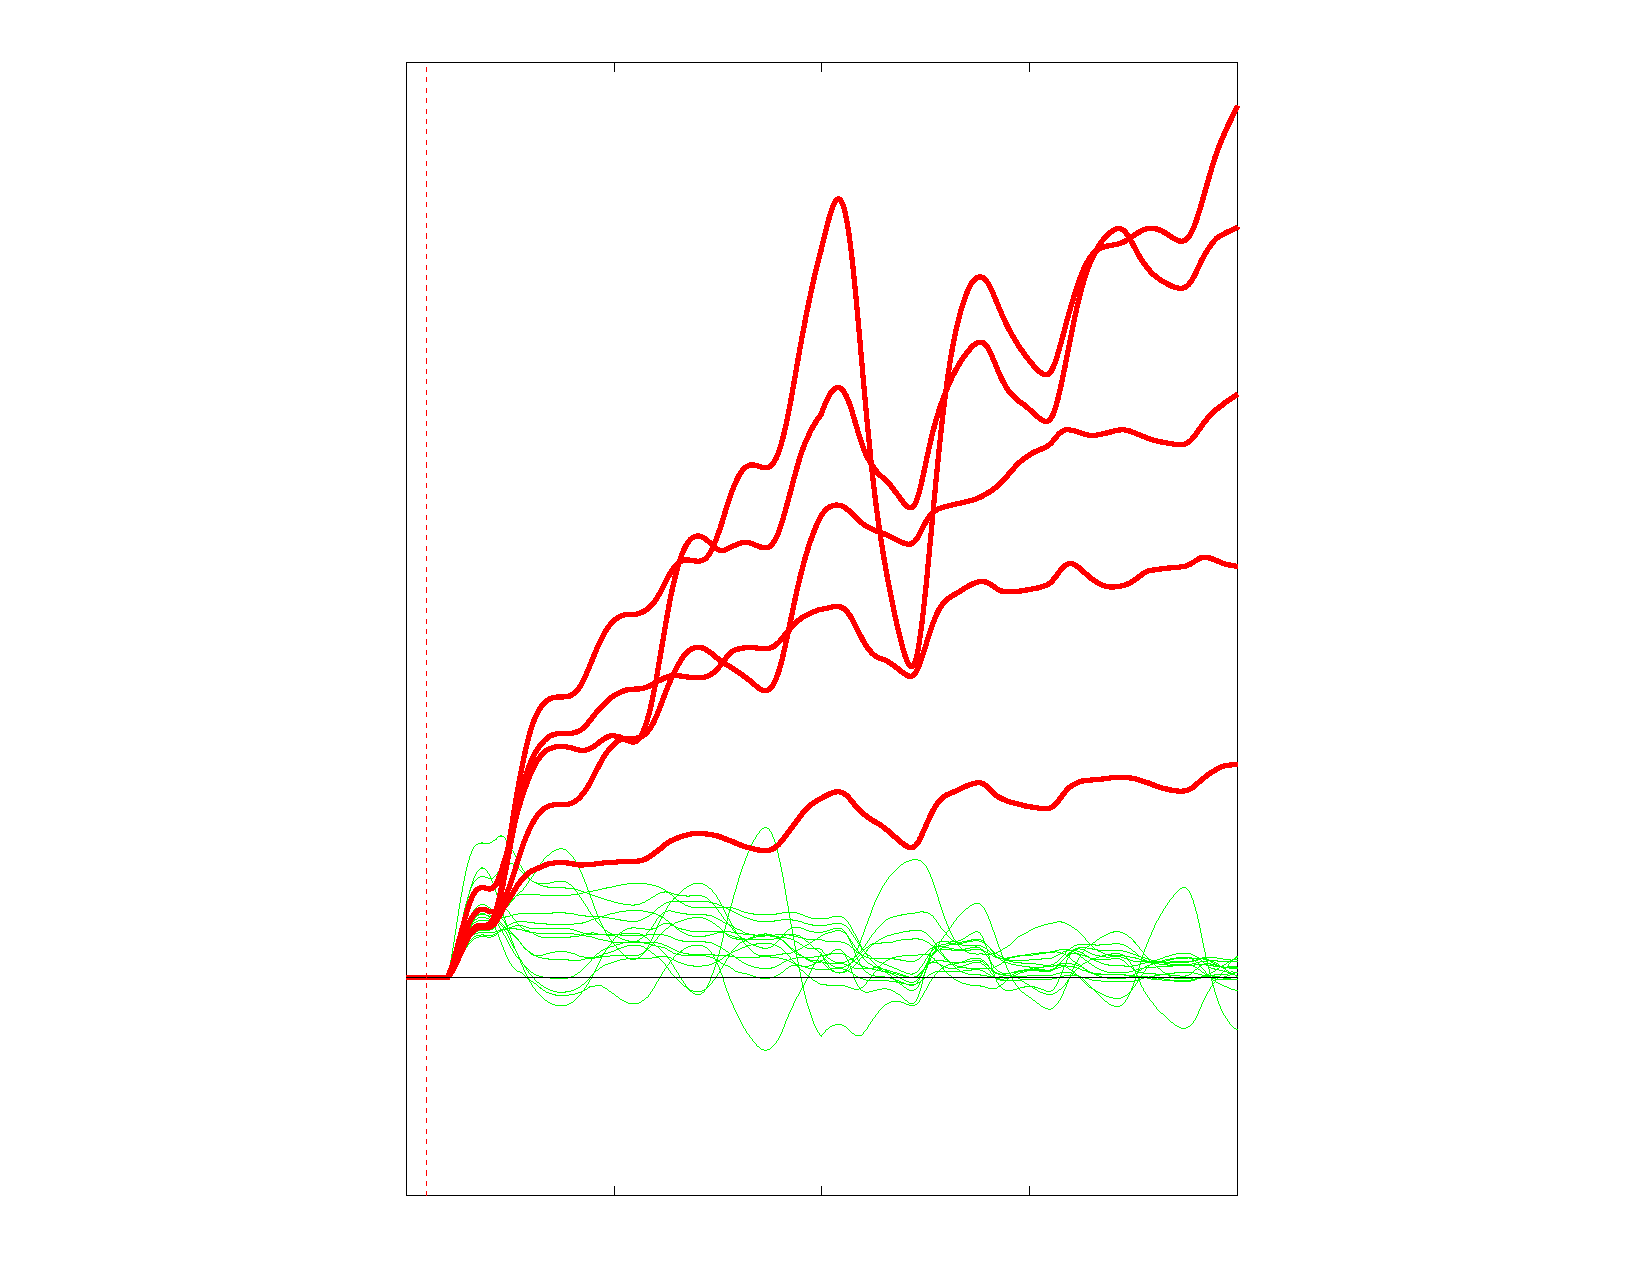
\includegraphics[trim={6.5cm 1cm 5cm 1cm},clip,width=6cm,height=3.5cm]{img/409-clusterSmallWorld-20-addUniform-40-spike5-gaussian-Unobserved-rank1-ukf-Xhat}};
\node at (-5.5,-0.25) {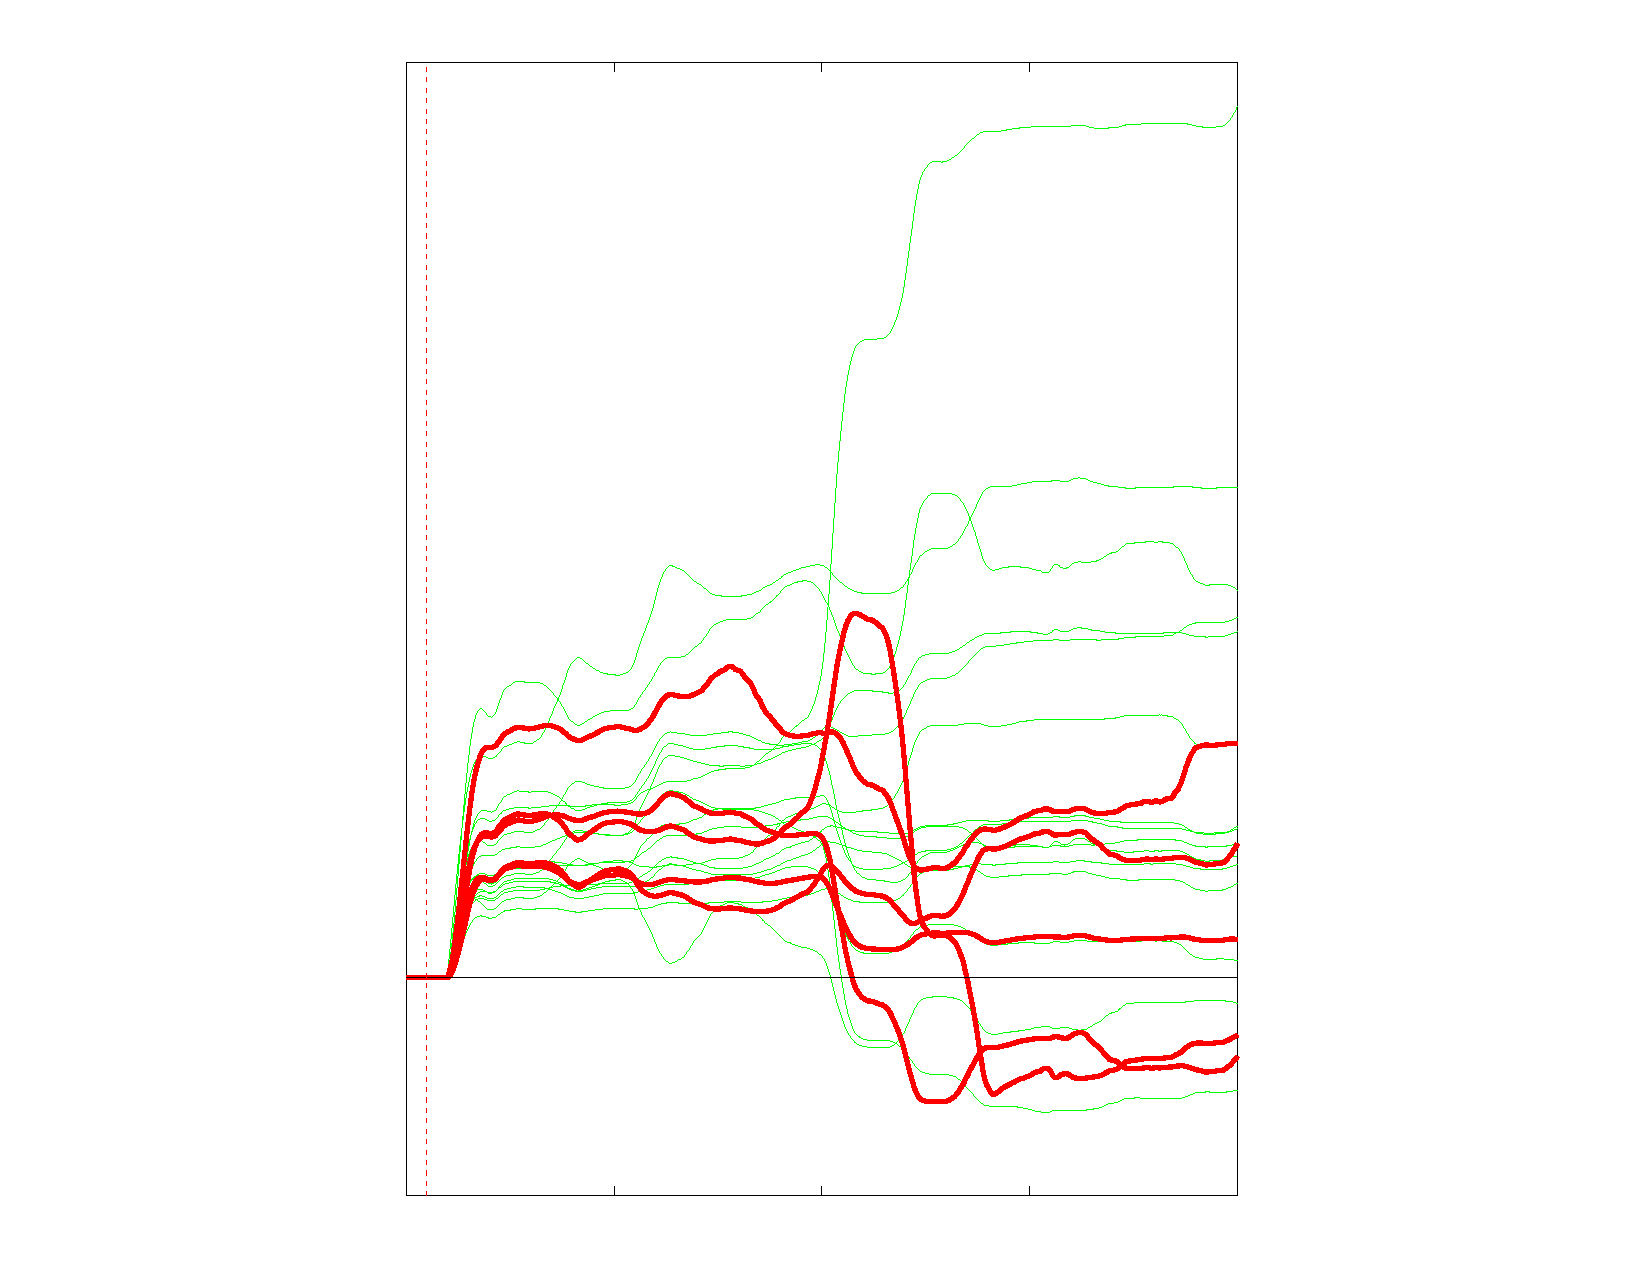
\includegraphics[trim={6.5cm 1cm 5cm 1cm},clip,width=6cm,height=3.5cm]{img/409-clusterSmallWorld-20-addUniform-40-spike5-gaussian-Unobserved-fullKL-ukf-Xhat}};
}

\node at (-5.755,2.0) {full rank $K^{LG}$};
\node at (-0.25,2.0) {rank-1 $K^{LG}$};
%\node at (-0.25,5.75) {3 compromised buses};
%\node at (5.25,5.75) {5 compromised buses};

%\draw (-8.25,-2.65) -- (-7.30,-2.65);
%\draw[->] (-4.2,-2.65) -- (7.75,-2.65);
\node at (-5.75,-2.65) {simulation time (sec)};

\node at (-8.35,-2.25) {0.0};
\node at (-7.05,-2.25) {0.5};
\node at (-5.75,-2.25) {1.0};
\node at (-4.45,-2.25) {1.5};
\node at (-3.25,-2.25) {2.0};

\node at (-6.75,1.25) {attack initiated};
\draw[->,darkgray] (-7.95,1.25) -- (-8.15,1.25);

\node at (-1.5,1.15) {\color{red} compromised };
\node at (-1.5,0.80) {\color{red} buses};
%\draw[->,red] (-6,3.95) -- (-6.15,4.15);

\node at (0.3, -1.6) {\color{darkgreen} uncompromised buses};
%\draw[->,green] (5.25,0.9) -- (5.5,0.8);
\end{tikzpicture}

\vspace{0.0755in}
The \textcolor{red}{red line} should be high and the \textcolor{darkgreen}{green lines} should be low.

\vspace{0.075in}
The rank-1 approximation outperforms the full rank estimator

\vspace{0.075in}
\uncover<2-3> {
    (even when the rank of $K^{LG}>1$)
}
\end{frame}

%%%%%%%%%%%%%%%%%%%%%%%%%%%%%%%%%%%%%%%%%%%%%%%%%%%%%%%%%%%%%%%%%%%%%%%%%%%%%%%%

\begin{frame}{Simulation results (identification accuracy)}

At any timestep $t$, our method has accuracy 1 if all the compromised buses have highest estimated $K^{LG}_t$ entries; otherwise the method has accuracy 0

\vspace{0.075in}
Repeat our experiment over 100 random configurations

\begin{center}
\scalebox{0.8}{
\begin{tikzpicture}
%\small
\node at (-0.1,0) {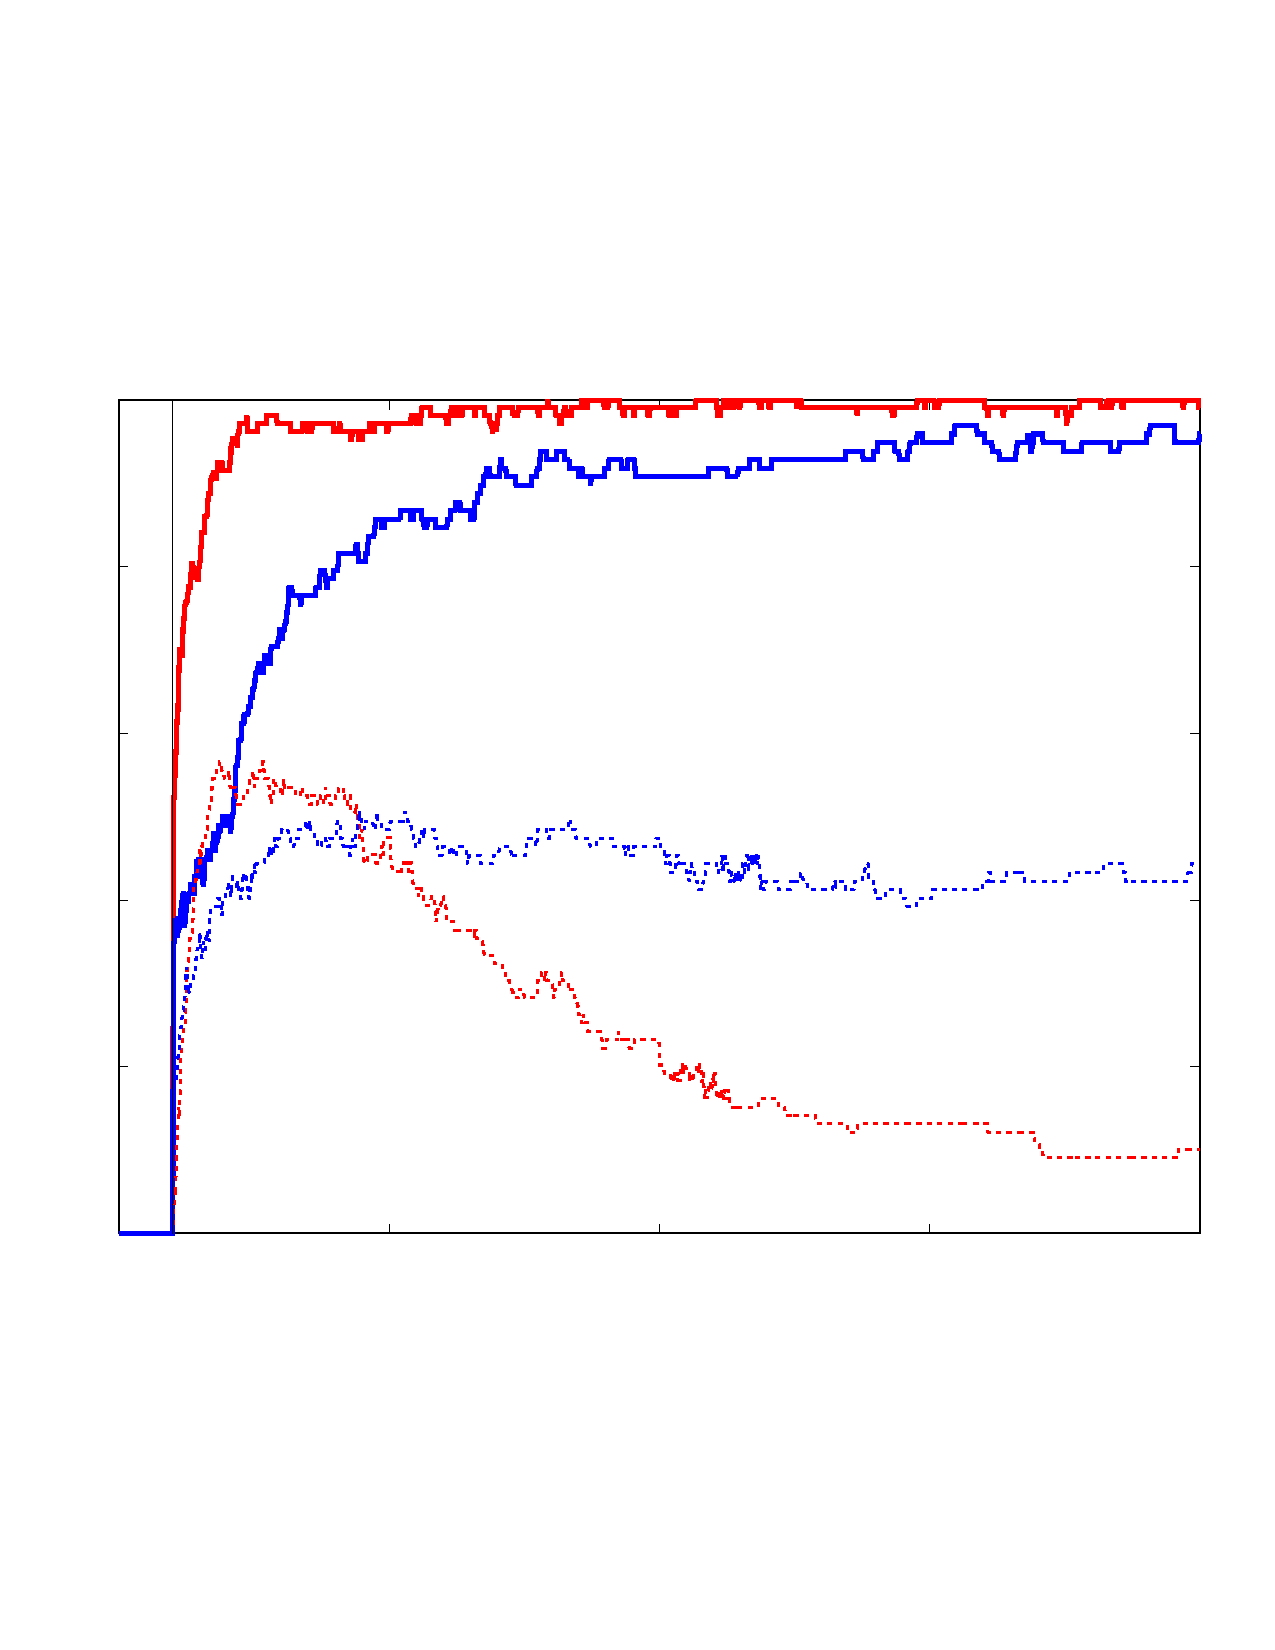
\includegraphics[trim={2cm 5cm 1cm 5cm},clip,width=7.2cm,height=7cm]{img/accuracy}};
\node at (0.0,-3.5) {simulation time (sec)};
\node at (-4.7,0) {\rotatebox{90}{accuracy of $\alpha_t$}};

\node at (-3.65,-3) {0.0};
\node at (-1.85,-3) {0.5};
\node at (-0.1,-3) {1.0};
\node at (1.65,-3) {1.5};
\node at (3.45,-3) {2.0};

\node at (-4.1,-2.7) { 0.0 };
\node at (-4.1,-1.6) { 0.2 };
\node at (-4.1,-0.5) { 0.4 };
\node at (-4.1,0.55) { 0.6 };
\node at (-4.1,1.65) { 0.8 };
\node at (-4.1,2.8) { 1.0 };

\node at (-1.7,-2.2) {\color{darkgray}attack initiated};
\draw[darkgray,->] (-2.9,-2.2) -- (-3.3,-2.2);

\node at (2,-1.5) {\color{red}\begin{tabular}{c}full $K^{LG}$\\1 compromised bus\end{tabular}};

\node at (2,0.25) {\color{blue}\begin{tabular}{c}full $K^{LG}$\\5 compromised buses\end{tabular}};

\node at (2,1.95) {\color{blue}\begin{tabular}{c}rank-1 $K^{LG}$\\5 compromised buses\end{tabular}};

\node at (-1.75,3.25) {\color{red}\begin{tabular}{c}rank-1 $K^{LG}$\\1 compromised bus\end{tabular}};

\end{tikzpicture}
}
\end{center}
\end{frame}


%%%%%%%%%%%%%%%%%%%%%%%%%%%%%%%%%%%%%%%%

\begin{frame}{Summary}
\Large
\begin{itemize}
\item Previous methods could only detect attacks

\vspace{0.15in}
\item New method for identifying system buses under attack
\vspace{-0.15in}
\begin{itemize}
\Large
\item joint estimation of system and attack parameters
\item solve with the Unscented Kalman Filter (UKF)
\end{itemize}

\vspace{0.15in}
\item Used a rank-1 approximation 
\begin{itemize}
\Large
\item better statistical efficiency
\item better computational efficiency
\end{itemize}
\end{itemize}

%\vspace{0.1in}
\begin{center}
\texttt{http://github.com/mikeizbicki/powergrid}
\end{center}

\pause
\begin{center}
{
\Huge
Questions?
}
\end{center}
\end{frame}

%%%%%%%%%%%%%%%%%%%%%%%%%%%%%%%%%%%%%%%%
\end{document}

